\documentclass{standalone}

\usepackage{tikz}
\usetikzlibrary{positioning}

\begin{document}
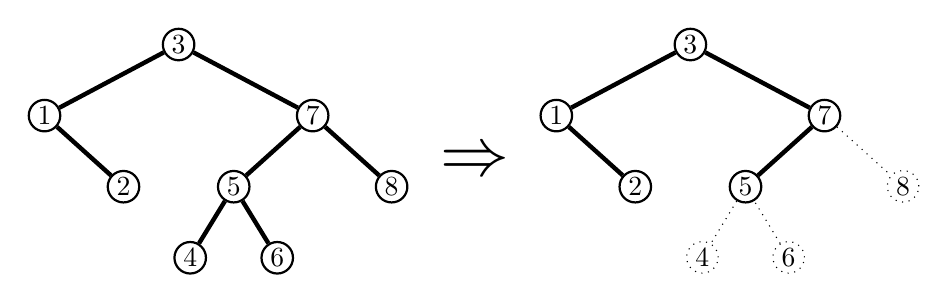
\begin{tikzpicture}[Tn/.style={draw,circle,minimum size=0.4cm, inner
  sep=0cm}, every node/.style={transform shape}]
  \node[Tn, thick] at (0,1.5) (a) {3};
\node[Tn, thick, below left=6mm and 14mm of a] (b) {1};
\node[Tn, thick, below right=6mm and 7mm of b] (c) {2};
\node[Tn, thick, below right=6mm and 14mm of a] (e) {7};
\node[Tn, thick, below right=6mm and 7mm of e] (f) {8};
\node[Tn, thick, below left=6mm and 7mm of e] (g) {5};
\node[Tn, thick, below left=6mm and 2.5mm of g] (h) {4};
\node[Tn, thick, below right=6mm and 2.5mm of g] (i) {6};

\draw[ultra thick] (c) -- (b) -- (a) -- (e) -- (f);
\draw[ultra thick] (e) -- (g) -- (h);
\draw[ultra thick] (g) -- (i);

\node at (3.7, 0) {\fontsize{30}{60} $\Rightarrow$};

\node[Tn, thick] at (6.5,1.5) (j) {3};
\node[Tn, thick, below left=6mm and 14mm of j] (k) {1};
\node[Tn, thick, below right=6mm and 7mm of k] (l) {2};
\node[Tn, thick, below right=6mm and 14mm of j] (m) {7};
\node[Tn, dotted, below right=6mm and 7mm of m] (n) {8};
\node[Tn, thick, below left=6mm and 7mm of m] (o) {5};
\node[Tn, dotted, below left=6mm and 2.5mm of o] (q) {4};
\node[Tn, dotted, below right=6mm and 2.5mm of o] (p) {6};

\draw[ultra thick] (l) -- (k) -- (j) -- (m) -- (o);
\draw[dotted] (m) -- (n);
\draw[dotted] (p) -- (o) -- (q);

\end{tikzpicture}
\end{document}
